% Please name the set of problems ubgXX.tex, and the solutions lsgXX.tex, where XX is the number

\documentclass[11pt]{article}
\usepackage[german]{babel}
\usepackage{epsfig,graphicx}
\usepackage{amsmath}
%\usepackage{axodraw}
\usepackage{mathrsfs}
\usepackage{amsfonts}
\usepackage{slashed}
%\usepackage{txfonts, pxfonts}
\textheight 240mm
\textwidth 168mm
\topmargin -1.5cm
\oddsidemargin -4mm
\evensidemargin -4mm
\pagestyle{empty}
\parindent 0mm

% Commands for typesetting of the exercises/solutions: please do not edit them
\newenvironment{questions}{\begin{list}{\alph{enumi})}{\usecounter{enumi}\leftmargin6mm}}{\end{list}}
\newcounter{exercise}
\newcommand{\exercise}[1]{\vspace{0.5cm}\stepcounter{exercise} \noindent {\large {\bf \arabic{exercise}. #1}}\\[1mm] }
%\newcommand{\serie}[2]{\noindent{{\bf \mbox{Exercises for Kern- und Teilchenphysik II --- Prof.\,F.\,Canelli, Prof\,N.\,Serra--- \\Spring term 2015 - Exercise sheet 1}}}\\
\newcommand{\serie}[2]{ \bf{Exercises for Kern- und Teilchenphysik II} \\ Prof.\,F.\,Canelli, Prof\,N.\,Serra \\Spring term 2015 - Exercise sheet 5\\
\rule{\linewidth}{0.3mm} \\ \noindent{\it Issued: 27 February 2015\\ Due: 5 March 2015  \\Discussion: 5 March 2015  }\\[2mm]
 }
\newcommand{\solutions}[1]{\noindent{ {\bf \mbox{Einf\"uhrung in die Kern- und Teilchenphysik --- Prof.\,K.\,Kirch --- Serie #1}}}\\\rule{\linewidth}{0.5mm} \noindent{\it L\"osungen }\\[2mm]}


% The following commands are defined for your convenience, they work in both math and text mode
\def\epem{\ensuremath{\mathrm{e^+e^-}}}      % e+e-
\def\TeV{\ensuremath{\mathrm{\ Te\kern -0.1em V}}} % TeV in correct typesetting
\def\GeV{\ensuremath{\mathrm{\ Ge\kern -0.1em V}}} % GeV in correct typesetting
\def\MeV{\ensuremath{\mathrm{\ Me\kern -0.1em V}}} % MeV in correct typesetting
\def\keV{\ensuremath{\mathrm{\ ke\kern -0.1em V}}} % keV in correct typesetting
\def\eV{\ensuremath{\mathrm{\ e\kern -0.1em V}}} % eV in correct typesetting
\def\tev{\TeV{}} % same as above, for convenience
\def\gev{\GeV{}}
\def\mev{\MeV{}}
\def\kev{\keV{}}
\def\ev{\eV{}}
\def\Wp{\ensuremath{\mathrm {W^+}}} % W+ boson
\def\Wm{\ensuremath{\mathrm {W^-}}} % W- boson
\def\ra{\ensuremath{\rightarrow}} %  "GOES TO" arrow for reactions
\def\rts {\ensuremath{\sqrt{s}}} % square root of s
\newcommand{\La}{\ensuremath{\mathcal{L}}}  % Luminosity
\newcommand{\p}{\ensuremath{\partial}} %

\begin{document}
%%%%%%%%%%%%%%%%%%%%%%%%%%%%%%%%%%%%%%%%%%%%%%%%%%%%%%%%%%%%%
%   Uncomment the appropriate line:
%
%\serie{1}{}  % insert (1) problem set number and (2) deadline here
%\serie{1}{1./3./4. M\"{a}rz 2011}  % insert (1) problem set number and (2) deadline here
%
%\solutions{1}  % insert solutions number here
%
%%%%%%%%%%%%%%%%%%%%%%%%%%%%%%%%%%%%%%%%%%%%%%%%%%%%%%%%%%%%%



%\begin{minipage}
%\fontsize{14pt}{12pt}\fontsize{10pt}{12pt}
\large
\textbf{
\centerline{Kern- und Teilchenphysik II}\\
\centerline{Spring Term 2015}\\
%\centerline{Prof.\,F.\,Canelli  Prof\,N.\,Serra}
\\
\Large \centerline{Exercise Sheet 5}
\\\\
}

\large
Lecturers: Prof.\,F.\,Canelli,  Prof.\,N.\,Serra\\
Assistants: Dr. M.\,Chrzaszcz, Dr. A.de Cosa

%Assistants: B. Casal Lara\~na, Dr. M. Doneg\`a, L. Tancredi, A. Torre\\
%\verb+https://moodle-app2.let.ethz.ch/course/view.php?id=1064+
%\end{minipage}
\normalsize


\exercise{$\tau$ lepton life time}

Assuming $\tau$ lepton decays only leptonic calculate the expected lifetime of the $\tau$ lepton. Check your calculations against the most precise experimental value~[HFAG 2014]:
\begin{equation}
\tau_{\tau} = (290.29 \pm 0.52)~\rm{ps}
\end{equation}
\begin{flushright}
3 pt
\end{flushright}

Why did we get a different result then experiments measured?
\begin{flushright}
1 pt
\end{flushright}


\exercise{Majorana fermions}

The most promising New Physics candidates are so called Majorana fermions. These particles are their own antiparticles and in the SM the only particles that can be majorana fermions are neutrinos. Why does this happen?”
\begin{flushright}
1 pt
\end{flushright}
Please show that the bispinor $\psi$ is Lorentz invariant under charge conjugate operator ($i \gamma^2$).
\begin{flushright}
2 pt
\end{flushright}
Let's write the bispinor as $\psi = (\psi_A, \psi_B)^T$. Please show that spinors $\psi_B$ and $\psi_A$ are not independent( use again the $i \gamma^2$ operator).
\begin{flushright}
2 pt
\end{flushright}
Why this happend? Why do we need just one component of bispinor to describe the full majorana neutrino system?
\begin{flushright}
1 pt
\end{flushright}


\exercise{Dark photon}

One of the candidate for new physics particle is so called dark photon. For this exercise let's assume that this is a massive! spin 0 particle for which we make the following QED rules:
\begin{enumerate}
\item Dark photon propagator:
\begin{equation}
\dfrac{-i}{q^2-(m_{\gamma}c^2)}
\end{equation}
\item Vertex factor is: $\emph{1}$
\end{enumerate}
Rest of its properties are identical as ''normal'' photon. Assuming it's kinematically allowed, calculate the decay rate of $\gamma_{dark} \rightarrow e^{-} e^{+}$
\begin{flushright}
3 pt
\end{flushright}
Find the lifetime of the dark photon assuming its mass to be $1~GeV/c^2$.
\begin{flushright}
1 pt
\end{flushright}
Write down the matrix element for a process: $e^{+} e^{-} \rightarrow \gamma_{dark} \gamma_{dark}$ (hint see figure below).
\begin{flushright}
3 pt
\end{flushright}

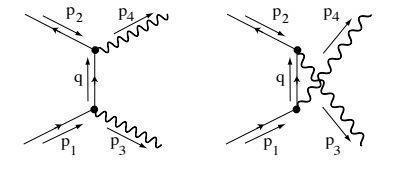
\includegraphics[width=0.4\textwidth]{dark.png}


Calculate $<|\mathcal{M}|>$ assuming the CM energy of electron position to be much larger then the photon and electron masses.
\begin{flushright}
3 pt
\end{flushright}

\end{document}
